% "{'classe':('PSI'),'chapitre':'cin_va','type':('td'),'titre':'Robot soudeur', 'source':'Pôle Chateaubriand - Joliot Curie','comp':(''),'corrige':True}"
%\setchapterimage{fig_00.jpg}
\chapter*{Application \arabic{cptApplication} \\ 
Robot soudeur  \ifnormal $\star$ \else \fi \ifdifficile $\star\star$ \else \fi \iftdifficile $\star\star\star$ \else \fi
 -- \ifprof Corrigé \else Sujet \fi}
\addcontentsline{toc}{section}{Application \arabic{cptApplication} : 
Robot soudeur  \ifnormal $\star$ \else \fi \ifdifficile $\star\star$ \else \fi \iftdifficile $\star\star\star$ \else \fi -- \ifprof Corrigé \else Sujet \fi}

\iflivret \stepcounter{cptApplication} \else
\ifprof  \stepcounter{cptApplication} \else \fi
\fi

\setcounter{question}{0}
\marginnote{Pôle Chateaubriand - Joliot Curie.}
\marginnote[1cm]{
%\UPSTIcompetence[2]{B2-14}
%\UPSTIcompetence[2]{C1-05}
%\UPSTIcompetence[2]{C2-07}
}

\begin{marginfigure}
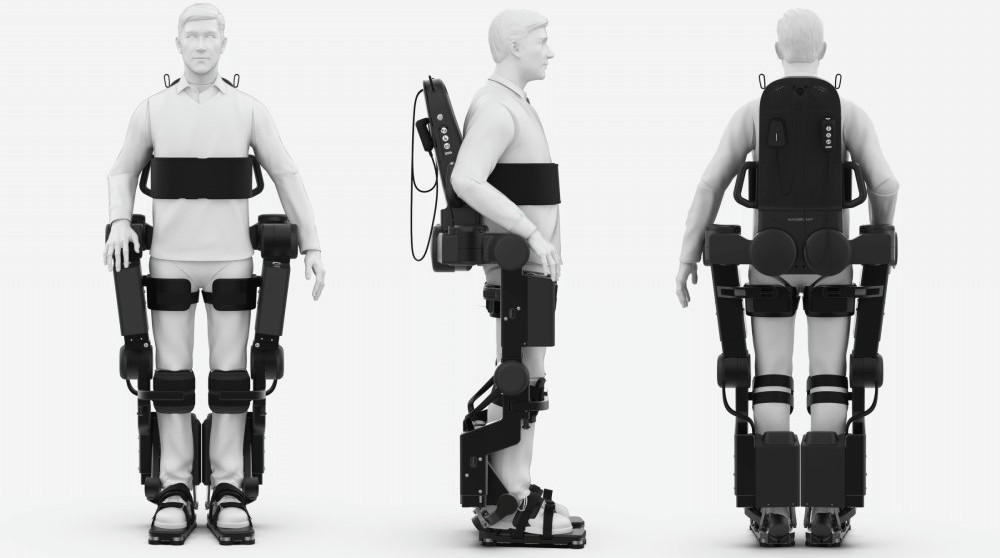
\includegraphics[width=\textwidth]{fig_00}
\end{marginfigure}


\subsection*{Mise en situation}

On s’intéresse à un robot soudeur dont le schéma cinématique lié à cette étude est proposé ci-dessous.
Sur ce schéma, les « flèches » au dessus des vecteurs unitaires ne sont pas représentées.


\begin{center}
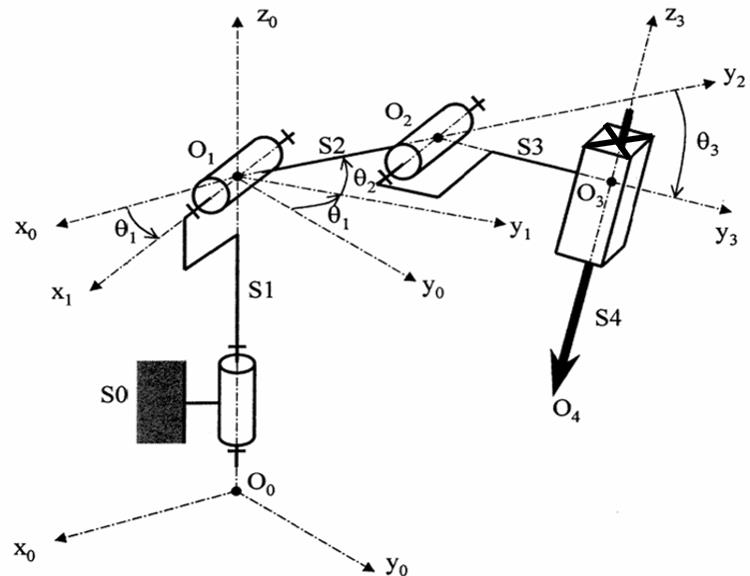
\includegraphics[width=.75\linewidth]{fig_1}
\end{center}

\begin{marginfigure}
\centering
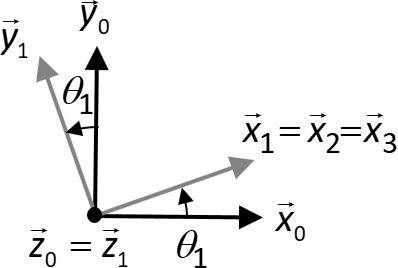
\includegraphics[width=.8\linewidth]{fig_2a}
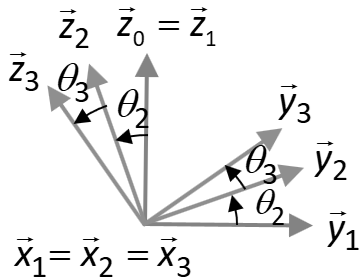
\includegraphics[width=.8\linewidth]{fig_2b}
\end{marginfigure}

Ce robot est constitué de cinq solides :
\begin{itemize}
\item le bâti 0, fixé au sol de l’atelier, de repère associé $\mathcal{R}_0=\left(O_0,\vect{x_0},\vect{y_0},\vect{z_0}\right)$ tel que $\vect{z_0}$ vertical ascendant ;
\item le fût 1, de repère associé $\mathcal{R}_1=\left(O_1,\vect{x_1},\vect{y_1},\vect{z_1}\right)$ tel que $\vect{z_1}  =\vect{z_0}$;
\item le bras 2, de repère associé $\mathcal{R}_2=\left(O_2,\vect{x_2},\vect{y_2},\vect{z_2}\right)$ tel que $\vect{x_1}  =\vect{x_2}$;
\item l’avant-bras 3, de repère associé $\mathcal{R}_3=\left(O_3,\vect{x_3},\vect{y_3},\vect{z_3}\right)$ tel que $\vect{x_2}  =\vect{x_3}$;
\item la buse 4, de repère associé $\mathcal{R}_4=\left(O_4,\vect{x_4},\vect{y_4},\vect{z_4}\right)$ tel que $\mathcal{B}_4  =\mathcal{B}_3$.
\end{itemize}


Chaque articulation possède son propre actionneur, le mouvement qui lui est associé peut donc être réalisé
indépendamment des autres.

\begin{multicols}{2}
\noindent Paramètres du mouvement :
\begin{itemize}
\item $\theta_1 = \angl{x_0}{x_1}$;
\item $\theta_2 = \angl{y_1}{y_2}$;
\item $\theta_3 = \angl{y_2}{y_3}$;
\item $\vect{O_3O_4} = \lambda \vect{z_3}$.
\end{itemize}

 \noindent  Caractéristiques géométriques :
\begin{itemize}
\item $\vect{O_0O_1} = L_1\vect{z_0}$;
\item $\vect{O_1O_2} = L_2\vect{y_2}$;
\item $\vect{O_2O_3} = L_3\vect{y_3}$.
\end{itemize}
$\quad$

\end{multicols}


Les figures de changement de base sont donnés ci-contre.


\noindent On donne ci-dessous un extrait du cahier des charges :
\begin{itemize}
\item exigence 1 : afin d’assurer la sécurité de l’environnement, la buse doit rester en permanence à l’intérieur
d’une sphère de centre $O_0$ et de rayon $R$.
\item exigence 2 : en phase d’utilisation normale, la buse doit se déplacer par rapport au bâti suivant la droite $\axe{O_0}{y_0}$ : réalisation d’un cordon de soudure linéaire.
\item exigence 3 : pour que le cordon de soudure linéaire suivant $\vect{y_0}$ soit correctement réalisé, l’orientation de la
buse 4 par rapport à la direction verticale doit être constante, et la vitesse de la buse doit être 
constante : $V$.
\end{itemize}

\begin{obj}
Déterminer les relations à imposer entre les valeurs instantanées des paramètres de mouvement et
de leurs dérivées lors de la réalisation d’un cordon de soudure.
\end{obj}

\question{Préciser une condition sur le vecteur position du point $O_4$ dans le repère lié à 0 qui traduit l’exigence Ex1 du
cahier des charges. En déduire une relation à imposer aux paramètres de mouvement.}



\ifprof
\else
\begin{marginfigure}
\centering

\includegraphics[width=3cm]{Cy_12_Ch_03_Application_05_RobotSoudeur_qr}
\end{marginfigure}
\fi


\question{Préciser deux conditions sur le vecteur position du point $O_4$ dans le repère lié à 0 qui traduisent l’exigence Ex2 du cahier des charges. En déduire une relation à imposer aux paramètres de mouvement.}

\question{Déterminer le torseur $\torseurcin{V}{4}{0}$ au point $O_4$ puis calculer $\vectg{O_4}{4}{0}$.}

\question{Déterminer le torseur $\torseurcin{V}{4}{0}_{\text{impose}}$ qui traduit l'exigence Ex3.}

\question{On se place dans le cas où le moteur de l’articulation entre 0 et 1 est arrêté dans la position $\theta_1=0$, traduire
alors la condition $\torseurcin{V}{4}{0}=\torseurcin{V}{4}{0}_{\text{impose}}$ en deux relations vectorielles.}

\question{En déduire 3 relations scalaires imposées entre les paramètres de mouvement et/ou leurs dérivées.}
